\section{Direkter digitaler Reglerentwurf}

Beim direkten Reglerentwurf wird die Strecke $G_S(s)$ in zeitdiskrete Form $\overline{G}_S(z)$ gebracht.
Anschliessend wird für $\overline{G}_S(z)$ ein (zeitdiskreter) Regler $G_{\rm R, D}(z)$ entworfen.


\subsection{Direkter digitaler Reglerentwurf -- Vorgehen}

Das Vorgehen und die Berechnungen sind grundsätzlich gleich wie im zeitkontinuierlichen Bereich, weshalb in folgender Abbildung der Platzhalter $\cdot$ für $s$ oder $z$ verwendet ist.
Es müssen jedoch einige Voraussetzungen erfüllt sein.

\vspace{-0.2cm}

\begin{center}
    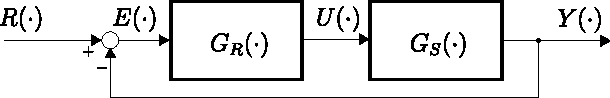
\includegraphics[width=0.75\columnwidth, align=t]{images/direkt_dig_reg_regelkreis.pdf}
\end{center}

$$ \text{Geschlossener Regelkreis} \quad  G_f(\cdot) = \frac{Y(\cdot)}{R(\cdot)} = \frac{G_S(\cdot) G_R(\cdot)}{1 + G_S(\cdot)G_R(\cdot)} $$


\subsubsection{Voraussetzungen}

\begin{outline}
    \1 Alle involvierten Teilsysteme müssen \textbf{'kompatibel'} sein
        \2 Entweder alles in $z$ formuliert oder alles in $s$ formuliert
    \1 Zeitdiskrete Systeme müssen \textbf{dieselbe Abtastzeit} haben
\end{outline}



\subsection{ZOH-Diskretisierung -- Überblick}
\label{ZOH-Diskretisierung -- Überblick}

Eine ZOH-Diskretisierung kann an einer UTF oder im Zustandsraum durchgeführt werden:

\vspace{-0.2cm}

\begin{center}
    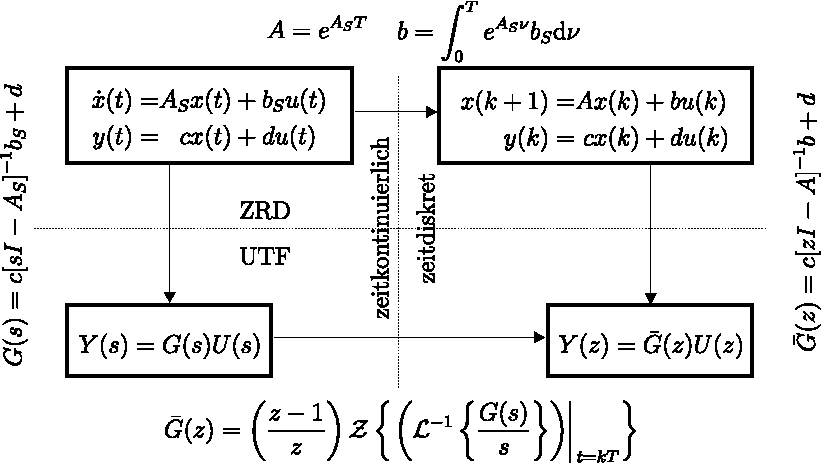
\includegraphics[width=0.9\columnwidth, align=t]{images/direkt_dig_reg_ZOH_konversion.pdf}
\end{center}

Beide Diskretisierungs-Arten werden in den Abschnitten \ref{ZOH-Diskretisierung mit UTF} und \ref{ZOH-Diskretisierung im Zustandsraum} genauer beschrieben.


\subsubsection{Steuerbarkeit / Beobachtbarkeit}{251-253}

Für Steuerbarkeit und Beobachtbarkeit bei der ZOH-Diskretisierung gilt:

\smallskip

\begin{outline}
    \1 Solange die Abtatzeit $T$ \textbf{sinnvoll gewählt} wird, bleiben diese Eigenschaften \textbf{erhalten}
    \1 Ein System kann durch Diskretisierung \textbf{nicht} steuerbar / beobachtbar \textbf{gemacht werden}
\end{outline}


\subsubsection{Stabilität}

Für die Stabilität gilt bei der ZOH-Diskretisierung:

\smallskip

\begin{outline}
    \1 Stabilität \textbf{bleibt} bei ZOH-Diskretisierung \textbf{erhalten}
        \2 Pole bzw. Eigenwerte gehorchen bei ZOH-Diskretisierung der Abbildung $z = e^{sT}$
\end{outline}

\smallskip


\paragraph{Abbildung $\bm{z = e^{sT}$}}

\begin{center}
    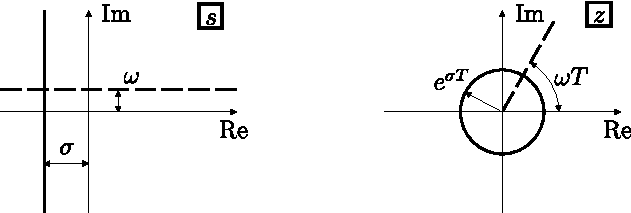
\includegraphics[width=0.8\columnwidth, align=t]{images/direkt_dig_reg_abbildung_geraden.pdf}
\end{center}


\begin{ctabular}{ccc}
    \toprule
    $\bm{s}$\textbf{-Ebene}             & \textlrarrow  & $\bm{z}$\textbf{-Ebene}       \\
    \midrule
    Gerade mit konstantem Imaginärteil  & \textlrarrow  & Halbgerade durch Nullpunkt    \\
    \midrule
    Geraden mit konstantem Realteil     & \textlrarrow  & Kreise um den Nullpunkt       \\
    \midrule
    Imaginärachse                       & \textlrarrow  & Einheitskreis                 \\
    \midrule
    Linke Halbebene                     & \textlrarrow  & Innerhalb des Einheitskreises \\
    \midrule
    Nullpunkt (Ursprung)                & \textlrarrow  & Punkt $(1 \, | \, 0)$         \\
    \bottomrule
\end{ctabular}


\example{Abblidung eines Streifens}

\begin{center}
    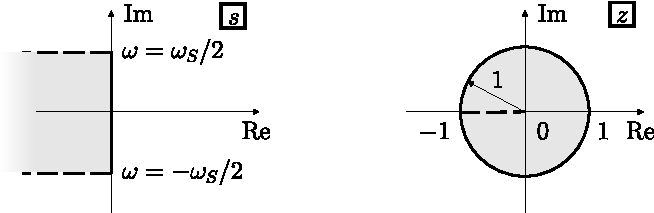
\includegraphics[width=0.8\columnwidth, align=t]{images/direkt_dig_reg_abbildung_beispiel.pdf}
\end{center}

\vspace{-0.2cm}


\subsection{ZOH-Diskretisierung mit UTF}{248-249}
\label{ZOH-Diskretisierung mit UTF}

Eine zeitkontinuierliche Strecke $G_S(s) = G(s)$ wird mit einem ZOH-Glied (zero-order-hold) \textbf{exakt} diskretisiert, weil der Eingang  zur zeitdiskreten Strecke als stückweise konstant angenommen werden kann.

\begin{minipage}[c]{0.78\columnwidth}
    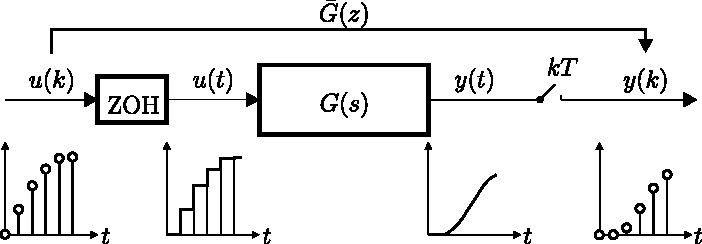
\includegraphics[width=\columnwidth, align=t]{images/direkt_dig_reg_ZOH_diskretisierung.pdf}
\end{minipage}
\hfill
\begin{minipage}[c]{0.2\columnwidth}
    $$ \overline{G}(z) = \frac{Y(z)}{U(z)} $$
\end{minipage}

\smallskip

Im Gegenzug zur ZOH-Diskretisierung ist die Approximation der Strecke mittels z.B. Tustin beim indirekten Reglerentwurf nicht exakt!


\subsubsection{Bestimmung der diskreten Stecke $\bm{\overline{G}_S(z)}$}

Die Bestimmung von $\overline{G}_S(z)$ wird vereinfacht durch Betrachtung der \textbf{Impulsantwort}. \\
Mit $u(k) = \{ 1, \, 0, \, 0, \, 0, \, \ldots \}$ ergibt sich am Ausgang die Impulsantwort $y(k) = g(k)$, deren \\
z-Transformierte $ G(z) \, (= \overline{G}_S(z))$ ist.

\smallskip

Als Formel kann die diskrete UTF $\overline{G}_S(z)$ ermittelt werden als:
\vspace{-0.2cm}
$$ \boxed{ \overline{G}_S(z)    = \left(\frac{z-1}{z} \right) \, \mathcal{Z} \left\{ \left( \mathcal{L}^{-1} \left\{ \frac{G_S(s)}{s} \right\} \right) \Bigg|_{t = kT} \right\}
                                = (1 - z^{-1}) \, \mathcal{Z} \left\{ \left( \mathcal{L}^{-1} \left\{ \frac{G_S(s)}{s} \right\} \right) \Bigg|_{t = kT} \right\} } $$
                       

\example{ZOH-Diskretisierung mit UTF}

Eine gegebene Strecke $G_S(s) = \frac{1}{s^2}$ soll mittels ZOH diskretisiert werden. 
Es soll also $\overline{G}_S(z)$ bestimmt werden, indem obige Formel Schritt für Schritt angewendet wird.
\vspace{-0.2cm}
\[
    \underbrace{ \frac{1}{s^2} }_{G_S(s)} \
    \underrightarrow{\div s} \quad 
    \frac{1}{s^3} \quad 
    \underrightarrow{\mathcal{L}^{-1}} \quad 
    \frac{t^2}{2} \quad
    \underrightarrow{t = kT} \quad 
    \frac{k^2 T^2}{2} \quad
    \underrightarrow{\mathcal{Z}} \quad 
    \frac{T^2}{2} \frac{z (z+1)}{(z-1)^3} \quad
    \underrightarrow{\cdot \left( \frac{z-1}{z} \right)} \quad 
    \underbrace{ \frac{T^2}{2} \frac{(z+1)}{(z-1)^2}}_{\overline{G}_S(z)}
\]

\vspace{-0.4cm}

\subsection{ZOH-Diskretisierung im Zustandsraum}{250-251}
\label{ZOH-Diskretisierung im Zustandsraum}

Eine zeitkontinuierliche ZRD kann in eine zeitdiskrete ZRD umgewandelt werden (entspricht dem Weg 'rechts herum' in Abschnitt \ref{ZOH-Diskretisierung -- Überblick}).
Die Variablen des Zustandsvektors bleiben bei der Diskretisierung erhalten, werden jedoch nur noch zum Abtastzeitpunkt evaluiert.

\smallskip

Die diskrete ZRD kann dargestellt werden als:

\vspace{-0.2cm}

\begin{minipage}[c]{0.4\columnwidth}
    \begin{align*}
        x(k+1)  &= \bm{A} \cdot x(k) + b \cdot u(k) \\
        y(k)    &= c \cdot x(k) + d \cdot u(k)
    \end{align*}
\end{minipage}
\hfill
\begin{minipage}[c]{0.58\columnwidth}
    \[
        \bm{A}  = e^{\bm{A_S} T} \qquad
        b       = \int\limits_0^T e^{\bm{A_S} \nu} \, \diff \nu \cdot b_S
    \]
\end{minipage}

\smallskip

\textbf{Hinweis:} $\bm{A_S}$ und $b_S$ entsprechen den zeit\myul{kontinuierlichen} ZRD-Werten 


\subsubsection{Bestimmung der diskreten Stecke $\bm{\overline{G}_S(z)}$}

Die diskrete UTF der Strecke $\bm{\overline{G}_S(z)}$ kann aus der diskreten ZRD ähnlich wie im zeitkontinuierlichen Bereich bestimmt werden:
\vspace{-0.2cm}
$$ \overline{G}_S(z) = c \cdot (z \bm{I} - \bm{A})^{-1} \cdot b + d $$


\subsection{Reglerentwurf -- WOK}{254}

Basierend auf den Pole / Nullstellen des offeren Regelkreises werden die Pole / Nullstellen des geschlossenen Regelkreises (bzw. die Pole des Reglers) platziert.
Da das Zeichnen der WOK (des \textbf{geschlossenen} Regelkreises) analog zum zeitkontinuierlichen Bereich erfolgt, wird dies hier nicht weiter erläutert (\textrightarrow\ siehe Anhang Abschnitt \ref{Wurzelortskurven (WOK)}).

\smallskip

Die (zeitdiskrete) UTF des geschlossenen Regelkreises mit einem P-Regler mit Verstärkung $K$ ergibt sich als
\vspace{-0.2cm}
$$ G_f(z) = \frac{K \cdot G_S(z)}{1 + K \cdot G_S(z)} = \frac{ K \cdot \frac{Z_S(z)}{N_S(z)} }{1 + K \cdot \frac{Z_S(z)}{N_S(z)}}
    = \frac{K \cdot Z_S(z) }{ \underbrace{N_S(z) + K \cdot Z_S(z) }_{\text{char. Polynom } N_f(s)} } = \frac{Z_f(z)}{N_f(z)} $$


Wird ein dynamischer Regler verwendet, so wird $G_0(z)$ in die \textbf{mathematisch verlangte Form} von aufgeteilt.
\vspace{-0.2cm}
$$ G_f(z) = \frac{G_R(z) \cdot G_S(z)}{1 + G_R(z) \cdot G_S(z)} = \frac{ \frac{Z_R(z)}{N_R(z)} \cdot \frac{Z_S(z)}{N_S(z)} }{1 + \frac{Z_R(z)}{N_R(z)} \cdot \frac{Z_S(z)}{N_S(z)}}
    = \frac{Z_R(z) \cdot Z_S(z) }{ \underbrace{N_R(z) \cdot N_S(z) + Z_R(z) \cdot Z_S(z) }_{\text{char. Polynom } N_f(s)} } = \frac{Z_f(z)}{N_f(z)} $$


\begingroup
\fbox{\parbox{0.97\columnwidth}{
    \raggedright
    \textbf{Hinweis:} Die Methode zur \textbf{Wurzel-Bestimmung} funktioniert für \textbf{jedes Polynom} $\bm{N_f(s)}$ (oder auch $N_f(z)$), wenn dieses in 
    die verlangte Form gebracht werden kann (und auch nur dann)!

    \vspace{-0.2cm}

    $$ N_f(s) = P_N(s) + \text{Faktor} \cdot P_Z(s) = N(s) + K \cdot Z(s) $$
}}
\endgroup

\smallskip

\textbf{Hinweis:} Wie eine WOK (in $s$) gezeichnet wird kann dem Anhang (Abschnitt \ref{Zeichnen von Wurzelortskurven}) entnommen werden.


\subsubsection{Platzierung der Pole}

\begin{outline}
    \1 Pole \textbf{innerhalb des Einheitskreises} platzieren ($\abs{z} < 1$)
    \1 Gebiet, welches Spezifikation erfüllt in z-Ebene transformieren und Pole innerhalb des transformierten Gebiets platzieren
    \1 Es können Interatoren (mit Polen bei $z = 1$) in den Regelkreis eingebaut werden
        \2 Somit wird der stationäre Fehler unterdrückt
\end{outline}


\subsection{Reglerentwurf -- Vorgabe des geschl. Regelkreises}{256-257}

Bei bekannter \textbf{diskreten} Regelstrecke $G_S(z)$ kann die benötigte UTF des Reglers $G_R(z)$ ermittelt werden, wenn die UTF des geschlossenen Regelkreises $G_f(z)$ vorgegeben ist.

\vspace{-0.2cm}

$$ G_f(z) = \frac{G_0(z)}{1 + G_0(z)} \quad \text{ \textlrarrow\ } \quad  G_0(z) = \frac{G_f(z)}{1 - G_f(z)}  \quad \text{und  } G_R(z) = \frac{G_0(z)}{G_S(z)}  $$


Daraus folgt für die UTF $G_R(z)$ des diskreten Reglers: 

\vspace{-0.1cm}

$$ \boxed{ G_R(z) = \frac{Z_f(z)}{N_f(z) - Z_f(z)} \cdot \frac{N_S(z)}{Z_S(z)} } \qquad \text{mit } G_S(z) = \frac{Z_S(z)}{N_S(z)} \text{ und  } G_f(z) = \frac{Z_f(z)}{N_f(z)} $$


\para{Bemerkungen}

\begin{outline}
    \1 Die Strecke $G_S(z)$ darf \textbf{keine} Pole ausserhalb des Einheitskreises haben
    \1 Die Strecke darf keine NS ausserhalb des Einheitskreises haben, ausser wenn dise in $G_f(z)$ übernommen werden
    \1 Die Strecke darf \textbf{Totzeiten} (ganzzahlige Vielfache der Abtastzeit) haben: $T_t = N \cdot T$
        \2 Stecke erhält dadurch $N$ zusätzliche Pole im Ursprung: $G_S(z) = \ldots \cdot z^{-N}$
    \1 Der relative Grad (\textbf{Polüberschuss}) der vorgegebenen UTF $G_f(z)$ muss mindestens so gross sein wie derjenige der Strecke $G_S(z)$
        \2 Regler ist sonst nicht realisierbar
\end{outline}
$$ \underbrace{ \mathrm{Ord}\{ N_S(z) \} - \mathrm{Ord}\{ Z_S(z) \} }_{\text{Polüberschuss Strecke}} \leq \underbrace{ \mathrm{Ord} \{N_f(z) \} - \mathrm{Ord} \{ Z_f(z) \} }_{\text{Polüberschuss geschl. System}} $$



\subsection{Reglerentwurf -- Deadbeat-Regler}{256-257}

Ein Deadbeat-Regler wird bei einem Führungsschritt der \textbf{Fehler in endlich vielen Abtastschritten Exakt zu Null}.
Der geschlossene Regelkreis $G_f(z)$ besetzt somit folgende Eigenschaften:

\begin{ctabular}{ll}
    \tabitem Alle Pole bei $z = 0$  & \tabitem Statische Verstärkung $G_f(1) = 1$
\end{ctabular}


\subsubsection{Einfachster Deadbeat-Regler}

Damit der Fehler zu Null, wird ist integrierendes Verhalten nötig. 
Der eifachste mögliche Regler $G_R(z)$ und der geschlossene Regelkreis $G_f(z)$ besitzen also die folgenden UTFs:

$$ G_R(z) = \frac{1}{z-1} \cdot \frac{1}{G_S(z)} \qquad \qquad \Rightarrow\ G_f(z) = \frac{1}{z} $$

Natürlich muss der Regler realisierbar sein (stabil, relativer Grad von $G_S$)


\subsection{Reglerentwurf -- Zustandsraum}{257-258}

Beim Reglerentwurf im Zustandsraum sind bei zeitdiskreten Systemen dieselben drei Komponenten von Interesse wie in zeitkontinuierlichen Systemen:

\smallskip

\begin{outline}
    \1 \textbf{Beobachter}, der den Zustandsvektor schätzt
    \1 \textbf{Zustandsrückführung}, die z.B. die Strecke stabilisiert
    \1 \textbf{Vorverstärkung}, für die statische Verstärkung \textrightarrow\ $G_f(1) = 1$
\end{outline}

\smallskip

Da die Konzepte weitgehend vom zeitkontinuierlichen Bereich übernommen werden können, werden nur ausgewählte Aspekte erwähnt.


\subsubsection{Polplatzierung}

\begin{outline}
    \1 Die Eigenwerte von $\bm{A} - \bm{BK}$ (und somit die Pole des Systems) ( \textrightarrow\ Zustandsrückführung) bzw. $\bm{A} - \bm{HC}$ ( \textrightarrow\ Beobachter) müssen nun innerhalb des Einheitskreises platziert werden
    \1 Es können dieselben Matlab-Funktionen verwendet werden wie bei einem zeitkontinuierlichen System
    \1 Separationsprinzip bleibt erhalten
\end{outline}


\subsubsection{LQR / LQG}

\begin{outline}
    \1 Es wird eine andere Zielfunktion $J$ optimiert, was zu einer anderen Ricatti-Gleichung führt
        \2 Mathematischer Lösungsweg ist anders
    \1 Matlab benötigt einen anderen Befehl: $\mylstbox{dlqr(...)}$ statt $\mylstbox{lqr(...)}$
\end{outline}


